\section{Method}\label{Method} 
For each VNTR locus $V$, and each read $R$, we have a binary classification function $f:V\times R\rightarrow\{0,1\}$, where $f(R,V)=1$ if and only if read $R$ maps to locus $V$. For each read and each of $N$ loci $V_1,\lodots,V_N$, our goal is to compute independent classification functions $f_i(V_i,R)$. Note that a read can be assigned to multiple VNTR loci, or to none. For this paper, we consider all the tandem repeats of the genome that appear in coding exons of the human genome ($N=1905$), as changes in coding VNTRs are highly likely to have a phenotypic effect. We use a simple, 2-layer feedforward Neural Network to compute $f_i$.

\subsection{Read Filtering.}
\MB{XXX}

\subsection{Neural Recruitment}
\paragraph{Training set.}
To train the model, we used ART next generation sequencing read simulator \cite{Huang2011} to generate 30X coverage reads from human reference genome with known locations, so the labels of reads is known. In addition, for each of the 1905 loci, we modified the number of repeats to be $\pm 3$ of the original count in the reference genome and simulated reads from those regions.

To do the experiments for each locus, we assigned the labels based on expected alignment regions and we randomly divided original set of reads into three parts: 70\% for training, 10\% for validation and 20\% for testing.

\paragraph{Embedding.}
% one-hot encoding of each k-mer
For a DNA string $w$ of length $k$, consider an bijection $\phi$ that maps $w$ to a unique number in $[0,4^k-1]$. Each read $R$ can be defined by a collection of overlapping $k$-mers. We use a one-hot encoding to map read $R$ to vector $v_R\in [0,1]^{4^k}$, such that $v_R[i]=1$ if and only if $\phi^{-1}(i) \in R$.

We set $k$ to 6 in this manuscript, except where we search for the optimal $k$ and compare the performance with respect to $k$.

\begin{figure}[ht]
% \vskip -0.1in
\begin{center}
\centerline{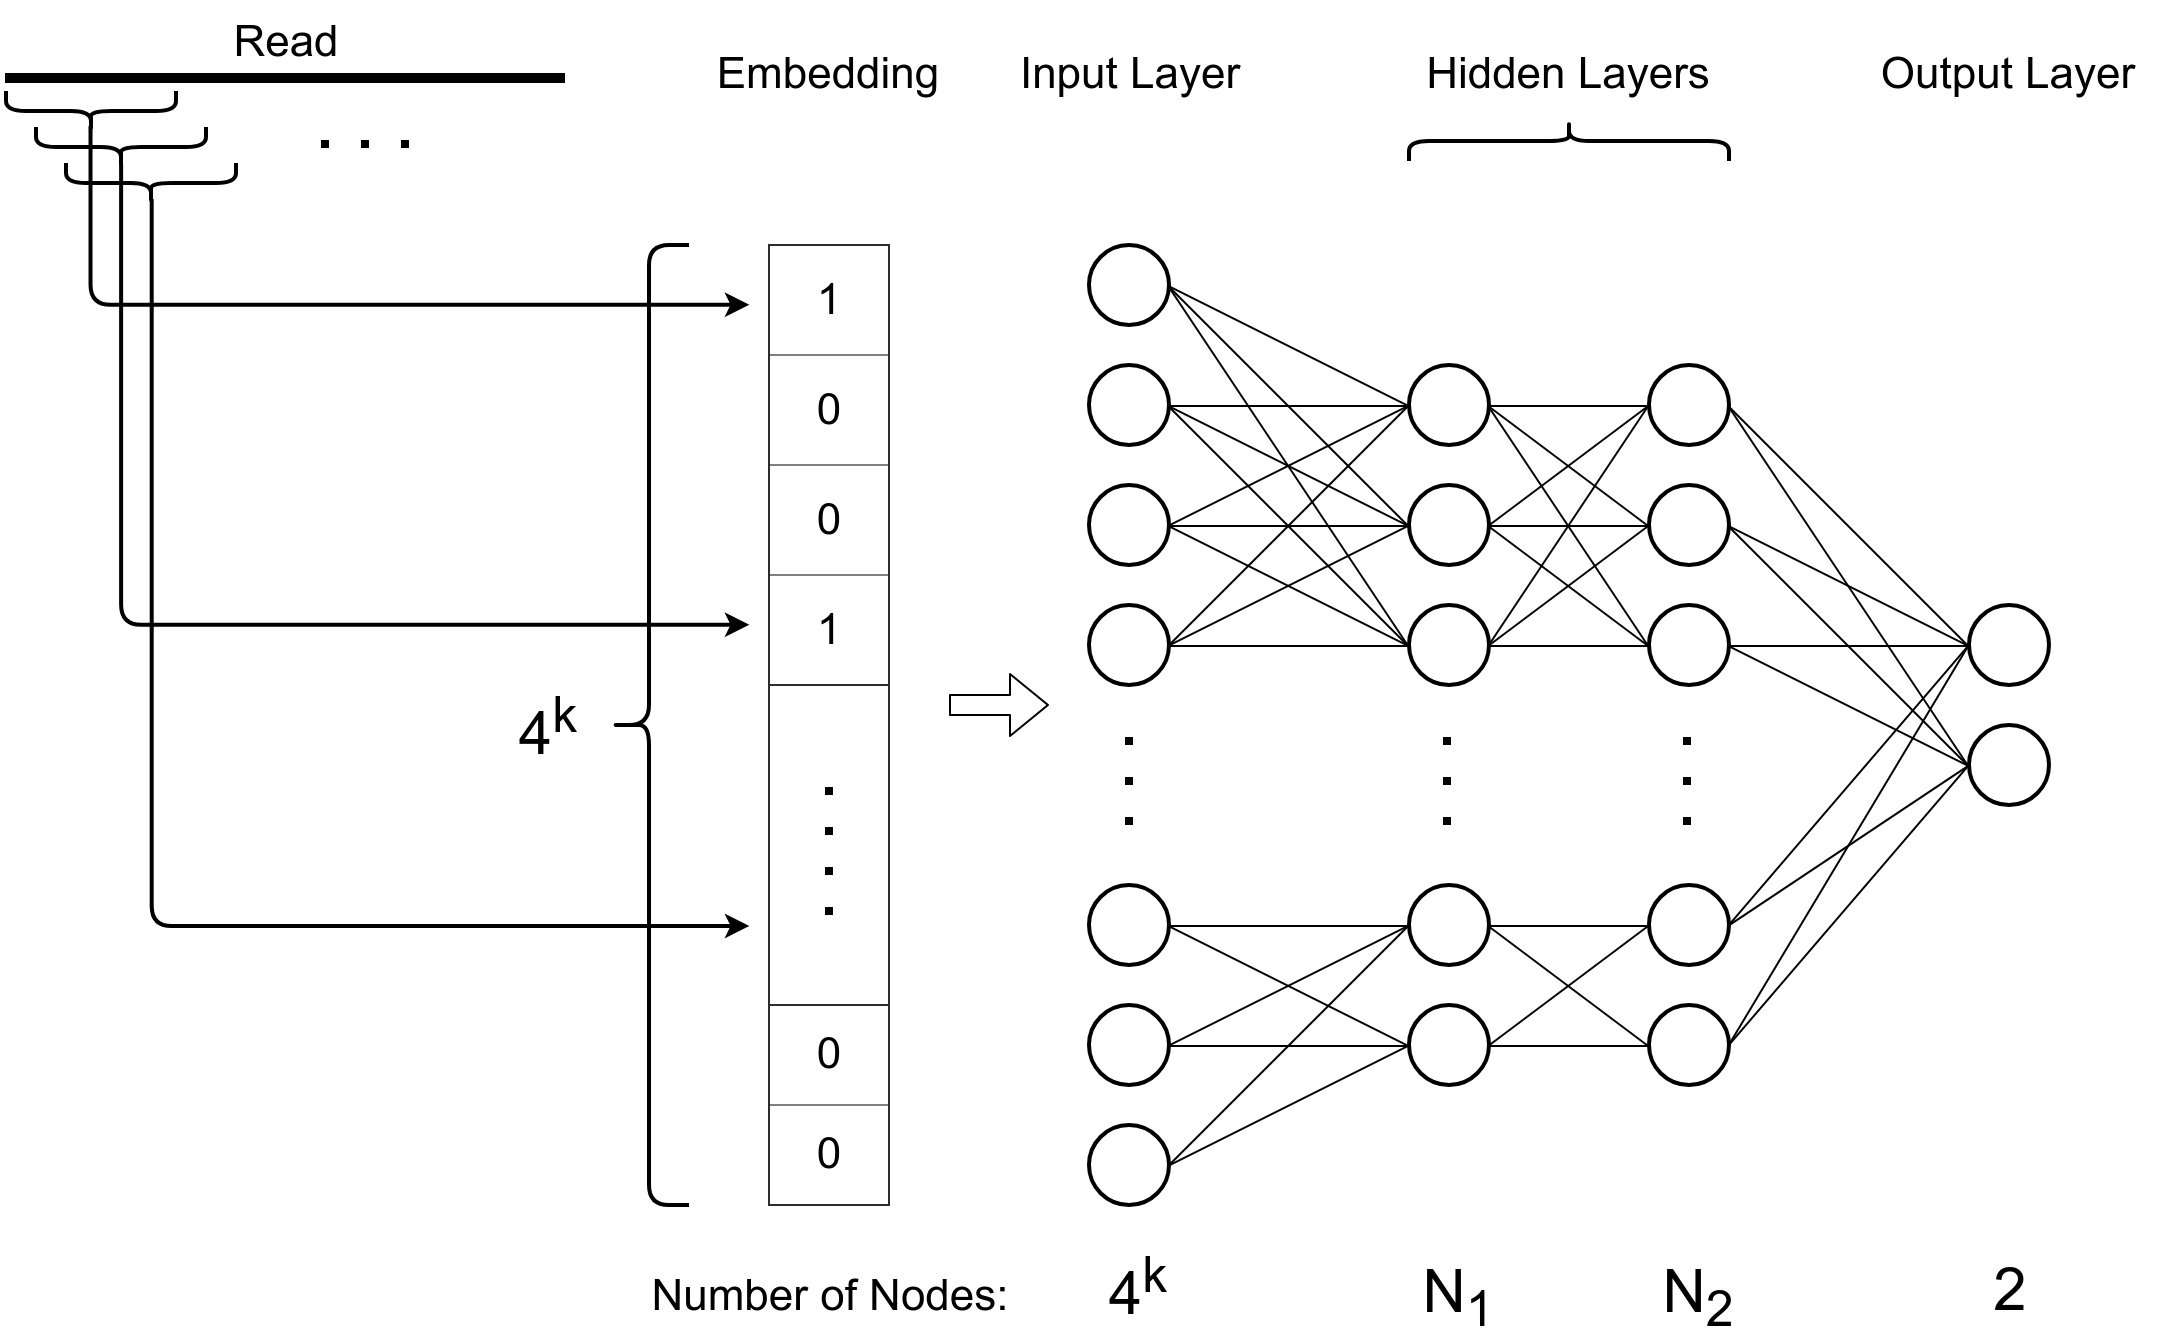
\includegraphics[width=\columnwidth]{fig/NeuralNetworkArch.png}}
  \caption{\footnotesize {\bf Neural Network Architecture.} Conversion of read sequence to vector of numbers, followed by network architecture.}
  \label{fig:neural_network}
\end{center}
\vspace{-0.3in}
\end{figure}

\paragraph{Regularization with noise.}
To form a regularization, we added random single nucleotide variations in the sequencing reads of dataset. For each read sequence in the dataset, we replaced its nucleotides with a random one with probability $r_e$\footnote{We set $r_e$ to the sum of sequencing error rate and novel mutation rate}. This method of dataset augmentation would also take care of nearby k-mers\footnote{A k-mer is a contiguous subsequence of k letters.} in the embedding of reads that may occur in the event of sequencing errors and novel mutations in different individual genomes. Hence, it would make the method more robust to having novel k-mers that are similar to the ones existing in the reference genome.

% Use Google Vizier for journal submission to find best parameters
\paragraph{Network Architecture.}
We present $v$ to the network via input layer.
We add two layers of fully connected nodes as the hidden layers such that every node is a \emph{Relu} function \cite{Nair2010}. In the output layer, there are two nodes $zero$ and $one$ which specify that whether read should be classified as true (containing VNTR) or false (Fig. ~\ref{fig:neural_network}). We used the training set to train the network with Adam optimization algorithm \cite{Kingma2014}.

The number of hidden layers $N_1$ and $N_2$ were chosen empirically. Too many nodes will increase both training time and test time and possibly cause over-fitting. We performed the training with the number hidden nodes of each layer varying from 10 to 100 with 10 increase in each step and selected $N_1=100$ and $N_2=50$ as the best parameters according to validation performance.

To choose the best loss function, we examined three regression loss functions Mean Squared Error (MSE), Mean Squared Logarithmic Error (MSLE), and Mean Absolute Error (MAE) as well as three binary classification loss functions Hinge, Squared Hinge, and Binary Cross-Entropy. Binary Cross-Entropy was chosen as the best loss function based on the performance on validation set (Results).

\subsection{VNTR Genotyping Pipeline}
Write about AWS, running time, and loci selection criteria.

\subsection{Identification of VNTR-eQTLs}
Linear model and p-value in 27 tissues.

\subsection{Fine-mapping of Causal Variants}
CAVIAR, p-value, ANOVA
